\documentclass[11pt]{article}

\usepackage[margin=1in]{geometry}
\usepackage{graphicx}
\usepackage{booktabs}
\usepackage[hidelinks]{hyperref}

\title{AthenaK STS Diffusion Benchmarks}
\author{AthenaK benchmark note}
\date{\today}

\begin{document}
\maketitle

\section{Goal}

This note compares explicit diffusion updates against super-time-stepping (STS) for the
three exact 1D diffusion problems currently maintained in AthenaK:
\begin{itemize}
  \item Hydro viscosity,
  \item Hydro thermal conduction,
  \item MHD Ohmic resistivity.
\end{itemize}

The comparison is CPU-only and uses the same exact problem generators already exercised by
the regression suite. The questions are simple:
\begin{itemize}
  \item Does STS preserve the same analytic accuracy as the explicit update?
  \item How much wall-clock time does STS save or cost on these exact problems?
\end{itemize}

\section{Setup}

All runs use the tracked exact diffusion inputs under \texttt{inputs/tests/}, a 1D
resolution sweep of $N_x = 64, 128, 256$, and the same final simulation time
$t = 4.0$. The exact Gaussian kernel in these tests is evaluated with the decks'
built-in offset $t_0 = 0.5$, so the analytic profile shown at the end of the run
corresponds to a kernel time of $t_0 + t = 4.5$.

Each benchmark point consists of one warm-up run plus five measured runs. The reported
runtime is the median wall-clock time over those five measured runs. The benchmark also
records AthenaK's printed \texttt{cpu time used}, \texttt{zone-cycles/cpu\_second}, final
cycle count, and first printed timestep. The fixed benchmark environment and the raw CSV
outputs live under \path{doc/data/sts_diffusion/}.

During a follow-up audit of the Hydro conduction case, AthenaK's explicit Hydro path was
updated to clear the face-flux scratch before appending explicit diffusion. This matters
for conduction because the operator writes only the energy-flux component. The results
reported here are from that corrected path and a rebuilt benchmark binary.

\begin{table}[ht]
\centering
\caption{Benchmark setup.}
\resizebox{\textwidth}{!}{\begin{tabular}{llllll}
\toprule
Case & PDE & EOS & Coefficient & STS cap & Resolutions \\
\midrule
Hydro viscosity & viscous diffusion of transverse velocity & Hydro ideal EOS & $\nu=1$ & none & 64, 128, 256 \\
Hydro conduction & thermal diffusion of internal-energy perturbation & Hydro ideal EOS & $\kappa=1$ & 4 & 64, 128, 256 \\
MHD resistivity & Ohmic diffusion of transverse magnetic field & MHD isothermal EOS & $\eta=1$ & 8 & 64, 128, 256 \\
\bottomrule
\end{tabular}
}
\end{table}

\section{Results}

Figure~\ref{fig:profiles} compares the highest-resolution numerical profiles against the
analytic solution. Figure~\ref{fig:frontier} shows the accuracy-cost frontier using median
wall time as the horizontal axis and the RMS $L_1$ error as the vertical axis.

\begin{figure}[ht]
\centering
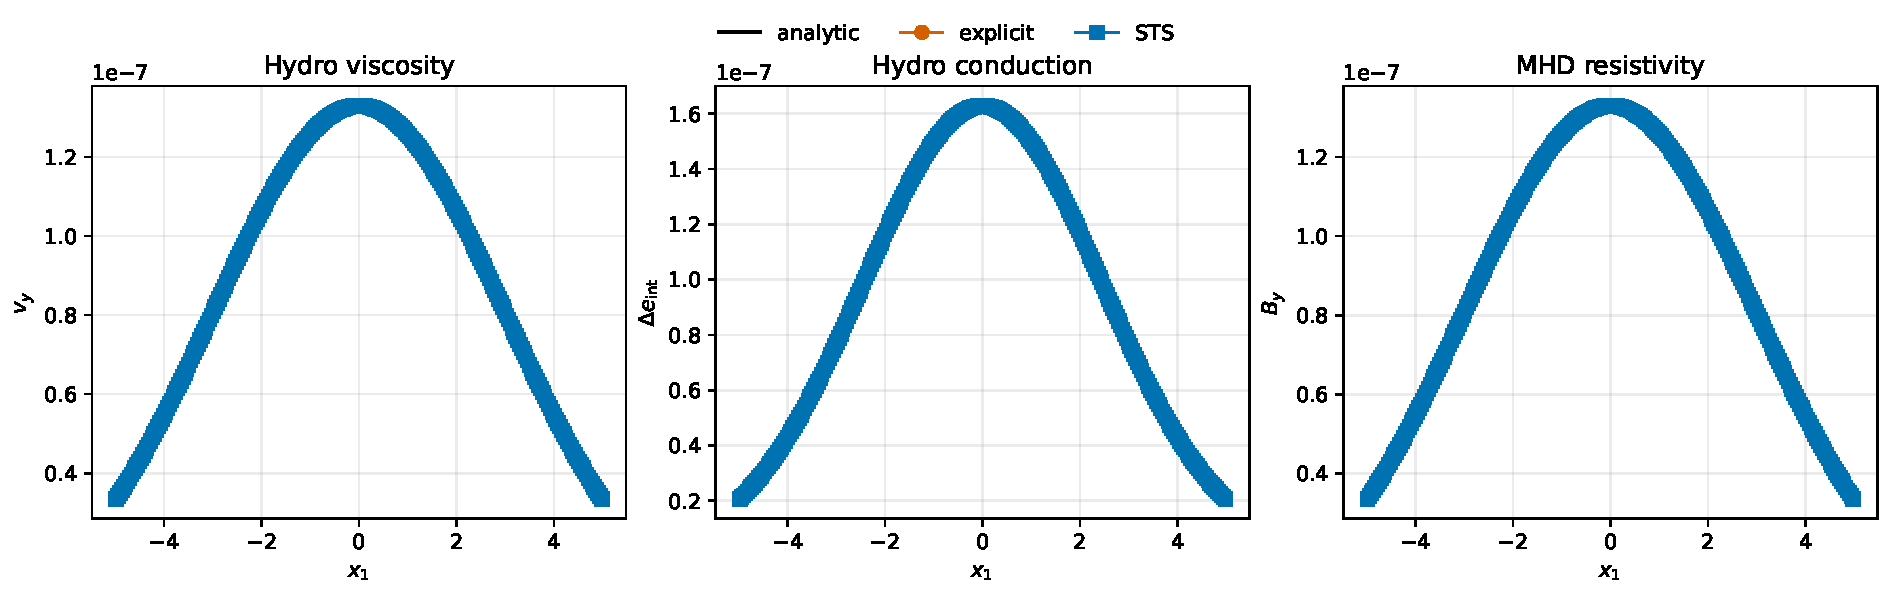
\includegraphics[width=\textwidth]{figures/sts_diffusion/sts_diffusion_profiles.pdf}
\caption{Highest-resolution profile comparison at $N_x = 256$. The conduction panel plots
the diffusing perturbation $\Delta e_{\rm int}$ after subtracting the constant background
internal energy.}
\label{fig:profiles}
\end{figure}

\begin{figure}[ht]
\centering
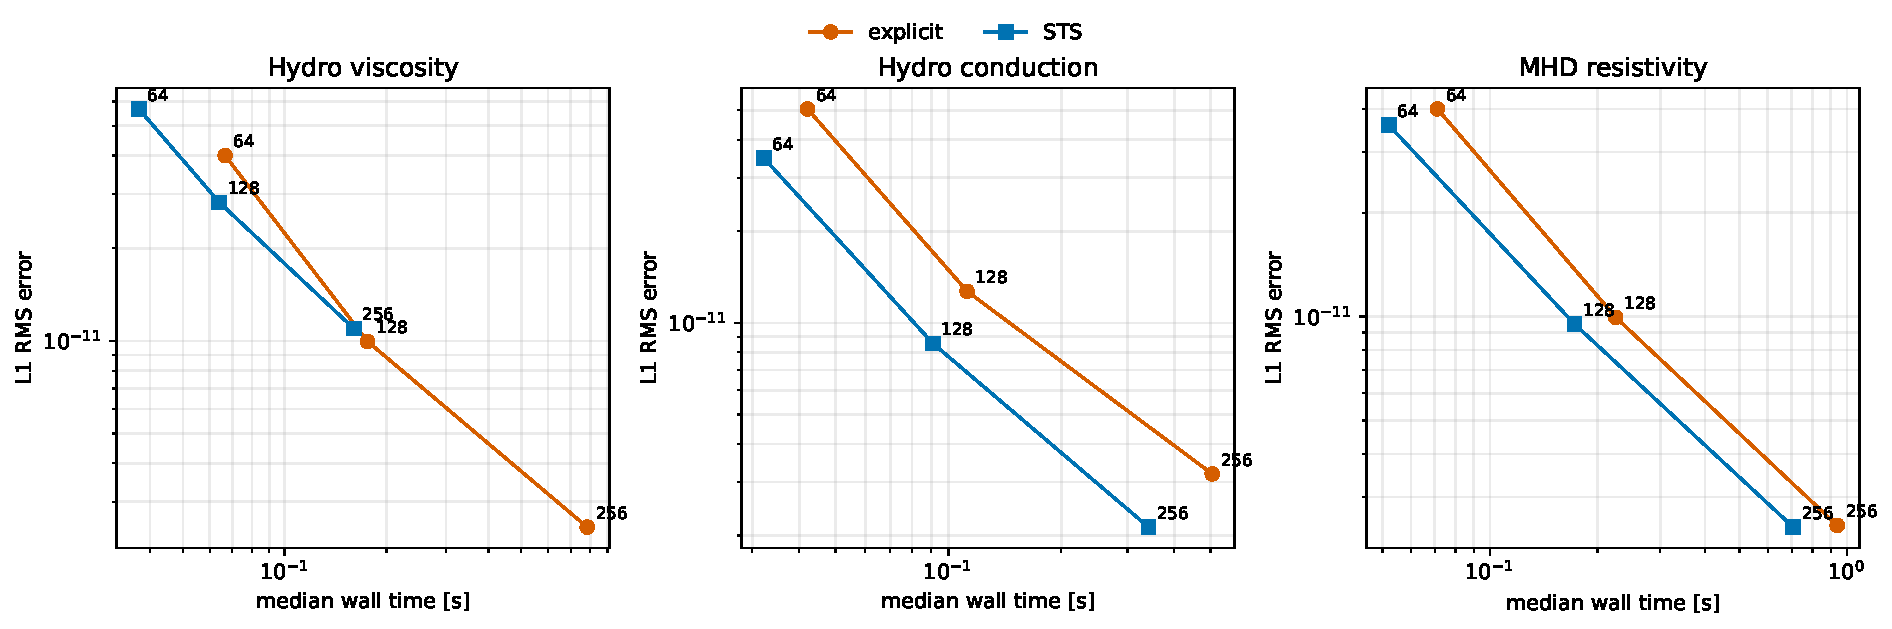
\includegraphics[width=\textwidth]{figures/sts_diffusion/sts_diffusion_accuracy_cost.pdf}
\caption{Accuracy-cost frontier for explicit and STS runs. Each point is labeled by the
1D resolution.}
\label{fig:frontier}
\end{figure}

\begin{table}[ht]
\centering
\caption{Highest-resolution matched comparison at $N_x = 256$. A speedup greater than 1
means STS is faster than the explicit run.}
\resizebox{\textwidth}{!}{\begin{tabular}{lrrrrrrr}
\toprule
Case & explicit RMS & STS RMS & STS/explicit & explicit $t$ [s] & STS $t$ [s] & speedup & cycles (exp/STS) \\
\midrule
Hydro viscosity & 2.482e-12 & 1.096e-11 & 4.417 & 0.783 & 0.160 & 4.895 & 13108/257 \\
Hydro conduction & 3.186e-12 & 2.130e-12 & 0.668 & 0.505 & 0.342 & 1.478 & 8739/2185 \\
MHD resistivity & 2.481e-12 & 2.455e-12 & 0.989 & 0.939 & 0.707 & 1.328 & 13108/1639 \\
\bottomrule
\end{tabular}
}
\end{table}

The highest-resolution comparison is:
\begin{itemize}
\item Hydro viscosity: at $N_x=256$, STS is 4.895x faster than the explicit run, while keeping the RMS error in the same small-error regime as explicit (1.096e-11 vs. 2.482e-12, ratio 4.417).
\item Hydro conduction: at $N_x=256$, STS is 1.478x faster than the explicit run, and a smaller RMS error than explicit (2.130e-12 vs. 3.186e-12, ratio 0.668).
\item MHD resistivity: at $N_x=256$, STS is 1.328x faster than the explicit run, with essentially the same RMS error as explicit (2.455e-12 vs. 2.481e-12, ratio 0.989).
\end{itemize}


\section{Conclusion}

For these exact 1D diffusion problems, STS preserves comparable analytic accuracy while
reducing wall-clock cost in all three cases measured here. The largest gain in this CPU
benchmark is Hydro viscosity, where STS cuts the runtime by a factor of about 4.8 while
keeping the RMS error at the same small $10^{-11}$ scale. Hydro conduction and MHD
resistivity both show more modest but still clear speedups while staying on the same
analytic solution as the explicit runs. In particular, the Hydro conduction case now
lands in the same small-error regime as the other exact tests after the Hydro explicit
flux-scratch fix described above.

The benchmark package in this note makes that comparison reproducible from the repository:
the driver script is \texttt{tst/scripts/diffusion/benchmark\_sts\_diffusion.py}, the
plotting script is \texttt{vis/python/plot\_sts\_diffusion\_benchmark.py}, and the
generated data products live under \path{doc/data/sts_diffusion/}.

\end{document}
